\documentclass[12pt]{article}
\usepackage{ucs}
\usepackage{graphicx}
\usepackage[utf8x]{inputenc} 
\usepackage[russian]{babel}  
\title{ Техническая книга, ФМЛ №30, команда А}
\begin{document}
	\maketitle
	\tableofcontents
	\newpage
	\section{Состав команды}
		\begin{itemize}
					\item Ильясов Александр
					\item Лутошкин Роман
					\item Поникаровский Антон
					\item Капитан: Жадковский Александр
		\end{itemize}
	\section{Стратегия}
		\subsection{Конструкция}
			\begin{enumerate}
					\item Робот должен быть мобильным, двигаться быстро и, по возможности в любом направлении (имеется в виду способность двигаться боком).
					\item Конструкция робота должна существенно упрощать оператору задачу, а не усложнять ее.
					\item Робот должен быть снабжен датчиками угла оборота (энкодерами) для лучшей управляемости в автономном периоде.
					\item Робот должен быть компактным и не занимать лишнего места, чтобы не мешать союзнику по альянсу, а также для удобства транспортировки.
					\item Робот должен быть способен управлять пятью (5) мячами одновременно.
					\item Робот должен иметь приспособление для перемещения подвижных корзин.
					\item По возможности робот должен быть легким, чтобы его было легче переносить
					\item Конструкция робота должна обеспечивать быстрый доступ ко всем его ключевым узлам.
			\end{enumerate}
	\section{Основная часть}
	\subsection{16.09.14}
		\begin{enumerate}
			\item Дата собрания : 16.09.14
			\item Цель:
				\begin{itemize}
					  \item Собрать основу робота, а именно колесную базу
					  \item Написать простейшую программу для управления роботом
				\end{itemize}			
			\item Реализация :
				\begin{itemize}
					\item Была собрана квадратная конструкция(Рис. 1)
					\item Написана программа для передвижения
				\end{itemize}
			\item Результаты
				\begin{itemize}
					\item Собран четырехколесный робот, способный передвигаться по четырем направлениям
					\item Робот управляется с помощью геймпада
				\end{itemize}
				Получившаяся конструкция:
				\begin{figure} [h]
					\centering
					\begin{minipage}{0.3\linewidth}
						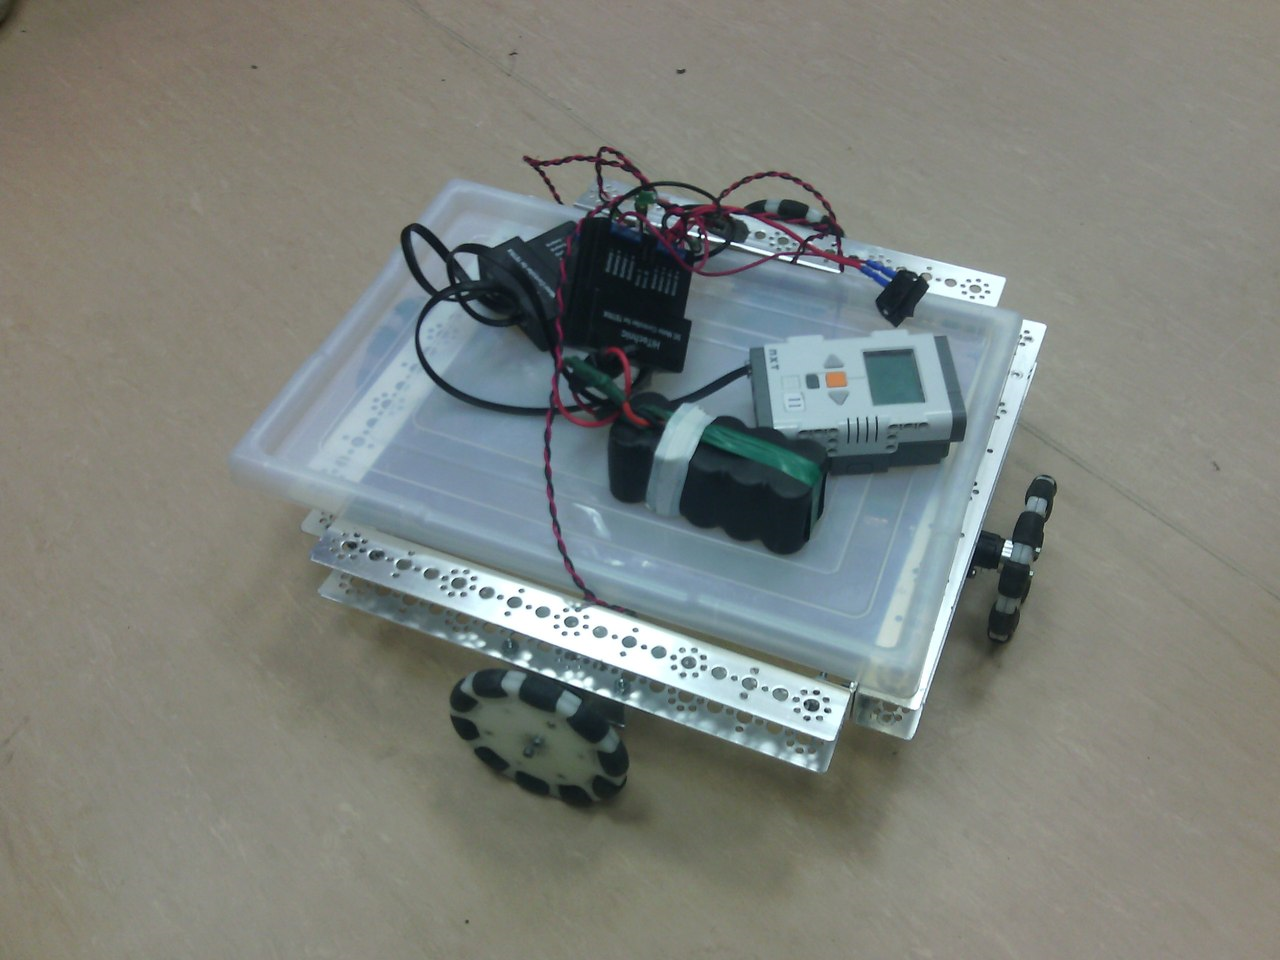
\includegraphics[width=40mm,height=40mm]{1_1_robot}\\ Рисунок 1
					\end{minipage}
					\begin{minipage}{0.3\linewidth}
						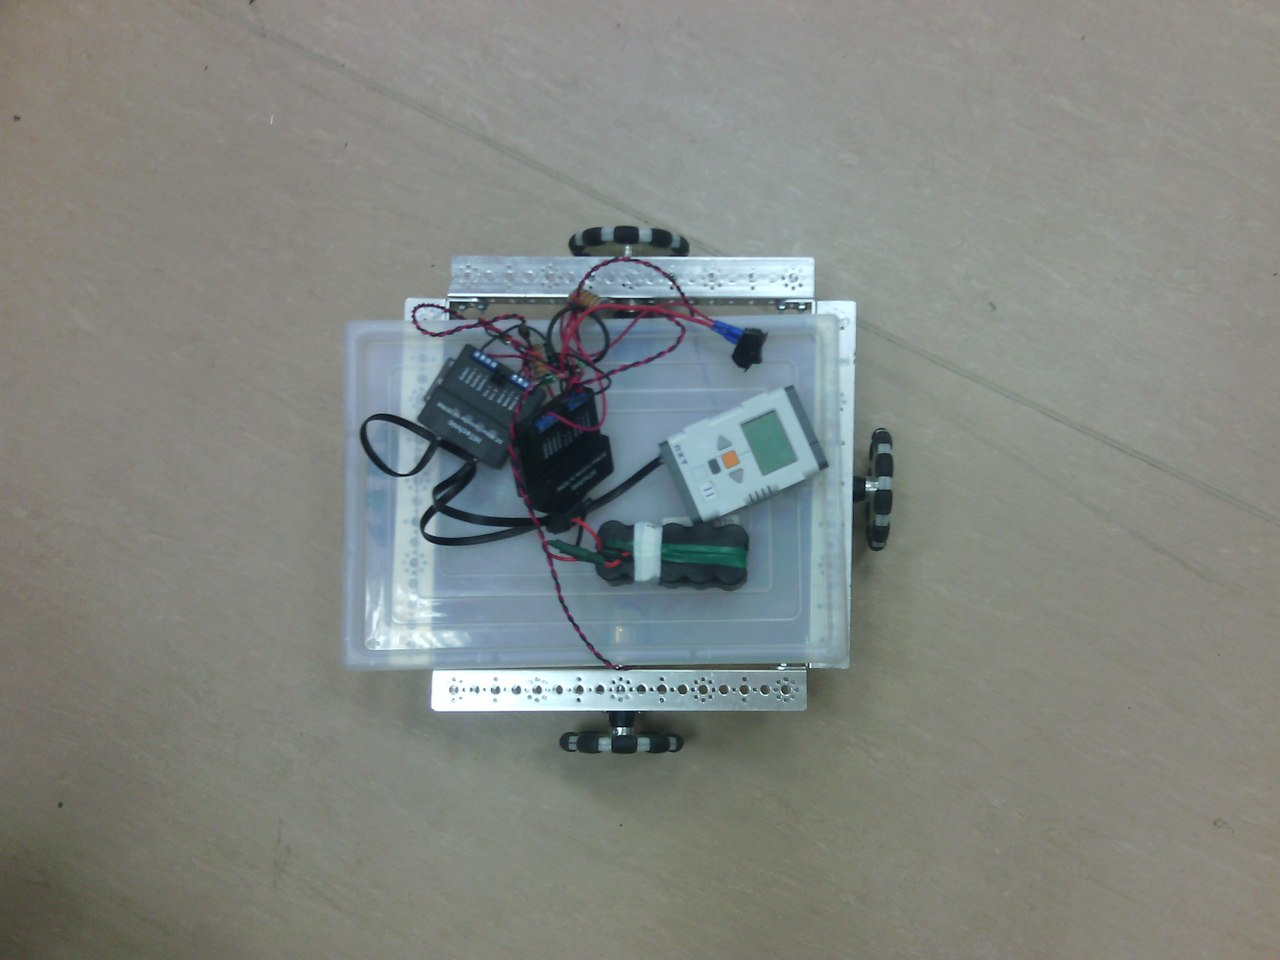
\includegraphics[width=40mm,height=40mm]{1_2_robot}\\ Рисунок 2
					\end{minipage}
				\end{figure}
		\end{enumerate}
	\newpage
	
	\subsection{3.10.14}
		\begin{enumerate}
			\item Дата собрания 3.10.14
			\item Цель:
				\begin{itemize}
					\item Укрепить конструкцию робота
					\item Разнести колеса по углам конструкции для увеличения площади колесной базы
					\item Закрепить основные узлы управления робота на конструкции с максимально легким доступом к к ним
					\item Оптимизировать программу, перенести управление передвижением робота с кнопок на джойстик
				\end{itemize}
			\item Результаты:
				\begin{itemize}
					\item Конструкция робота была укреплена, центр тяжести снижен 
					\item Двигатели были закреплены по углам конструкции, одновременно закрепляя ее
					\item На осях был закреплен второй ряд колес определенным образом для лучшего управления(Рисунок 2,3)
				\end{itemize}
			\begin{figure} [h]
				\centering
				\begin{minipage}{0.3\linewidth}
					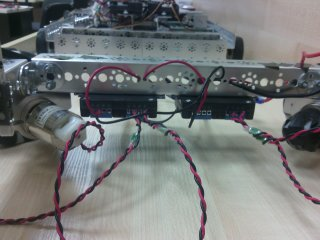
\includegraphics[width=40mm,height=40mm]{3_1_robot}\\ Рисунок 3
				\end{minipage}
				\begin{minipage}{0.3\linewidth}
					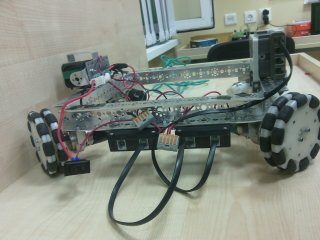
\includegraphics[width=40mm,height=40mm]{3_2_robot}\\ Рисунок 4
				\end{minipage}
				\begin{minipage}{0.3\linewidth}
					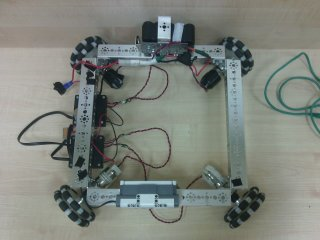
\includegraphics[width=40mm,height=40mm]{3_3_robot}\\ Рисунок 5
				\end{minipage}
			\end{figure}
			\item Идеи и планы для следующего занятия:
				\begin{itemize}
					\item Начать строить механизм захвата и подъема шариков. В качесте механизма подъема можно использовать ножничный подъемник, механизм захвата еще обдумывается
				\end{itemize}
		\end{enumerate}
		\newpage
		
		\subsection{17.10.14}
			\begin{enumerate}
				\item Дата собрания : 17.10.14
				\item Цель:
						\begin{itemize}
							\item Реализовать ножничный подъемник, механизм, приводящий его в движение и закрепление на кострукции робота
							\item Написать программу для управления захватом с отдельного геймпада
						\end{itemize}
					
				\item Результаты:
					\begin{itemize}
						\item Робот был частично разобран из-за недостатка деталей, была собрана примерная схема механизма передвижения подъемника(Рисунок 6)
						\item Написать и отладить программу не получилось, опять же из-за отсутствия деталей
					\end{itemize}
				\item Идеи:
					\begin{itemize}
						\item Заменить текущие рейки в подъемнике на алюминиевые профили для удобства установки, увеличения длины составляющих подъемника и уменьшения веса конструкции
						\item Отказаться от омниколес, поставить 4 обычных колеса
					\end{itemize}
			\end{enumerate}	
\end{document}